\section{Bestimmung des Planckschen Wirkungsquantums}
\subsection{Versuchsaufbau}
Um mithilfe des Photoeffekts\cite[S.78-80]{Demtröder:829119} das Plancksche Wirkungsquantum h zu bestimmen wird der
in \cref{fig:photozelle_optikbank} skizzierte Aufbau auf einer Optikbank befestigt.
Als Lichtquelle dient eine Quecksilberdampflampe, deren Licht nach Durchgang durch eine
Blende, mit der die Intensität des Lichts eingestellt werden kann,
mit einer Linse der Brennweite $f=\SI{100}{\milli\meter}$ auf die Kalium-Kathode
der Photozelle scharf abgebildet wird. Die einzelnen Wellenlängen des Hg-Spektrums
werden mithilfe eines Filterrads unmittelbar vor der Photozelle selektiert,
wobei zwischen beiden Elementen ein Rohr angebracht wird, welches Streulicht
begrenzen soll. Dabei wird das Lichtbündel mit der Blende vor der Lampe sowie der Blende vor
dem Filterrad so eingestellt, dass das Licht die Kathode beleuchtet, jedoch nicht
den Anodenring oder die schwarze Fläche an der Öffnung der Schutzkappe der Photozelle.\\

Zur Spannungserzeugung steht ein \SI{12}{\volt} Netzteil zur Verfügung. Beide schwarzen
Kabel der Anode werden an den negativen Pol des Netzteils angeschlossen und
das BNC-Kabel der Kathode mit dem zur Verfügung stehenden Messverstärker verbunden.
Der andere Anschluss des Netzteils wird an die Masse des Verstärkers angeschlossen.
Der Photostrom wird mit einem Digitalmultimeter gemessen, welches in Reihe hinter
den Verstärker geschaltet wird.
Die angeschlossene Grenzspannung wird mit einem parallel zur Spannungsquelle
geschalteten Multimeter gemessen.\\

Es ist möglich, dass ohne Photostrom der Verstärker trotzdem einen Strom ausgibt.
Mithilfe eines Tasters lässt sich die Schaltung kurzschließen, wodurch kein Strom
am Verstärker ankommt und damit an einem Regler der Ausgangsstrom in die Nulllage
kalibriert werden kann.\\

Da die vom Netzteil zu Verfügung stehenden \SI{12}{\volt} nicht vollständig in der Durchführung
ausgeschöpft werden, wird mit zwei geeigneten Widerständen ein Spannungsteiler
vorgeschaltet. Wird über dem Widerstand $R_2$ die Spannung abgegriffen, so gilt für diese
die Spannungsteilergleichung
\begin{equation}
	U = U_0\frac{R_2}{R_1 + R_2}
	\label{eq:spannungsteiler}
\end{equation}



\begin{figure}[htb]
	\centering
	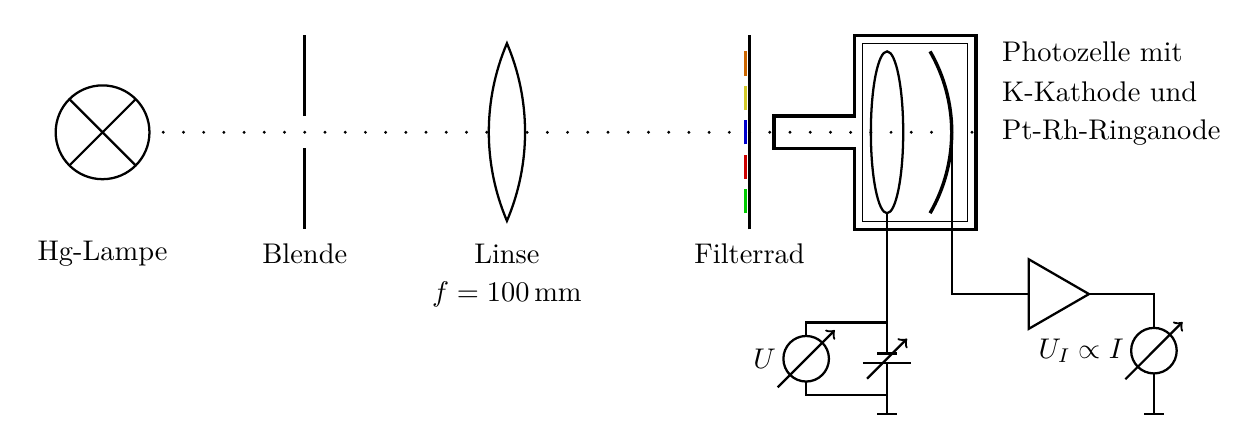
\includegraphics[width=0.8\linewidth]{../figs/photozelle_optikbank}
	\caption{Versuchsaufbau: Photoelektrische Bestimmung des planckschen Wirkungsquantum.
	\cite[S.19]{skript}}
	\label{fig:photozelle_optikbank}
\end{figure}

\subsection{Messung}
Im Folgenden wird mit $U$ die am Spannungsteiler abgegriffene Spannung bezeichnet und der Photostrom
mit $I$. Der Messverstärker wandelt Ströme von \SI{1}{\nano\ampere} in \SI{1}{\volt} um,
weshalb zwar mit dem Multimeter eine Spannung gemessen wird, diese trotzdem mit einem $I$ bezeichnet
wird. Der Strom entsteht, wenn energiereiche Photonen auf die Kathode treffen und
Elektronen befreien, die von der Anode wieder abgefangen werden.\\
Beide Elektroden besitzen verschiedene Austrittsarbeiten, weshalb sich die Fermi-Niveaus
dieser unterscheiden. Bei leitender Verbindung gleichen sich die Niveaus an, wodurch
ein elektrisches Feld zwischen den Elektroden aufgebaut wird
\cite{wiki:kontaktpotential}. 
Die Energiebilanz der eintreffenden
Elektronen ist
\begin{equation}
	E_\mathrm{kin} = \mathrm h\nu - (\mathrm W_{\mathrm A} - \mathrm W_{\mathrm K})
	- \mathrm W_{\mathrm K} = \mathrm h\nu - \mathrm W_{\mathrm A}\nonumber
\end{equation}
wobei das Subskript K für die Kathode, A für die Anode und $\nu$ für die Lichtfrequenz steht.
Mit dem Netzteil wird eine Gegenspannung eingestellt und so lange erhöht, bis
der Anodenstrom verschwindet. In diesem Falle verschwindet die kinetische Energie der Elektronen
und es ergibt sich bei der Grenzspannung $U_0$ die Gleichung
\begin{equation}
	\mathrm eU_0 = \mathrm h\nu - \mathrm W_{\mathrm A}
	\label{eq:gegenfeldmethode}
\end{equation}
mit dem Planckschen Wirkungsquantum\cite[S.75]{Demtröder:829119} 
$$\mathrm h=\SI{6.626e-34}{\joule\second}$$ 
auf drei Nachkommastellen gerundet sowie der Elementarladung\cite[S.29]{Demtröder:829119}
\[\mathrm e = \SI{1.602e-19}{\coulomb}\]
ebenfalls auf drei Nachkommastellen genau.

\begin{figure}[htb]
	\centering
	\begin{subfigure}[c]{0.46\linewidth}
		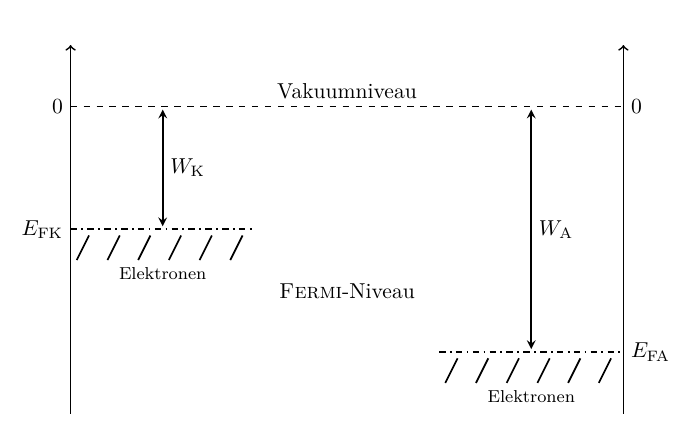
\includegraphics[width=\linewidth]{../figs/fermi1.png}
		\subcaption{nicht verbunden}
	\end{subfigure}
	\begin{subfigure}[c]{0.46\linewidth}
		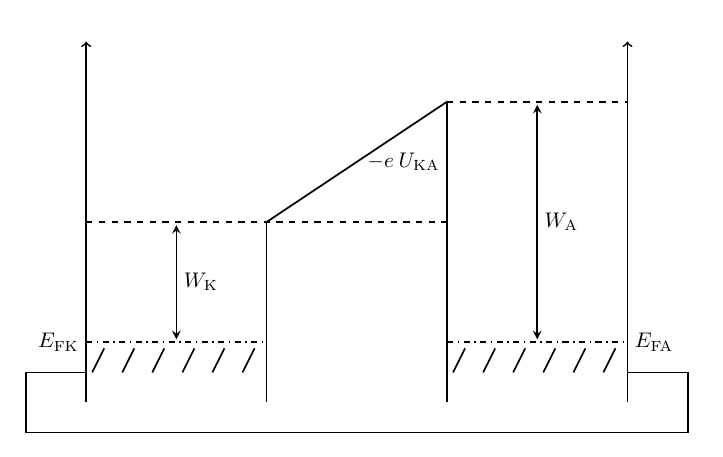
\includegraphics[width=\linewidth]{../figs/fermi2.png}
		\subcaption{leitend verbunden}
	\end{subfigure}
	\caption{Kontaktpotential zwischen zwei Elektroden}
\end{figure}

Bei dem energiereichsten Licht der Wellenlänge \SI{365}{\nano\meter} wird eine Grenzspannung von unter
\SI{2.0}{\volt} benötigt, weshalb mit den vorhandenen Widerständen von \SI{100}{\ohm} und \SI{333}{\ohm}
nach \cref{eq:spannungsteiler} eine maximale Spannung von
\[\mathrm U_\mathrm{max} = \SI{2.77}{\volt}\]
eingestellt wird.\\
Aufgrund dessen, dass ein minimaler Anodenstrom $I_0$ auch vorhanden ist, wo Elektronen aus der
Anode in die Kathode eintreffen, wird die Messung verfälscht. Um die Grenzspannung bestimmen zu können,
wird für jede Wellenlänge einen Kennlinie im gesamtem Gegenspannungsbereich gemessen, angefangen
bei \SI{0}{\volt}. Da zusätzliche Intensitätsfluktuationen auftreten können, wird jede Kennlinie
zweimal gemessen.\\\par
Für die Wellenlänge \SI{365}{\nano\meter} wird die Messung bei einer erhöhten Intensität
erneut gemessen, um den Einfluss der Lichtintensität auf die Kennlinie zu untersuchen.

\subsection{Auswertung}

\begin{figure}[htbp]
   \centering
\caption{Kennlinie \SI{365}{nm}}
\begin{tabular}{cc||cc}
\hline\multicolumn{2}{c||}{erste Messung} & \multicolumn{2}{c}{zweite Messung}\\

\hline
$U / \unit{\milli\volt}$ & $I / \unit{\pico\ampere}$ & $U / \unit{\milli\volt}$ & $I / \unit{\pico\ampere}$ \\ 
\hline
$\num{0}$ & $\num{732\pm 3}$ & $\num{0}$ & $\num{732\pm 4}$ \\
$\num{107}$ & $\num{638\pm 4}$ & $\num{120}$ & $\num{613\pm 4}$ \\
$\num{203}$ & $\num{556\pm 2}$ & $\num{242}$ & $\num{510\pm 3}$ \\
$\num{343}$ & $\num{436\pm 5}$ & $\num{381}$ & $\num{402\pm 2}$ \\
$\num{439}$ & $\num{375\pm 5}$ & $\num{497}$ & $\num{321\pm 1}$ \\
$\num{572}$ & $\num{282\pm 2}$ & $\num{615}$ & $\num{250\pm 1}$ \\
$\num{721}$ & $\num{198\pm 2}$ & $\num{733}$ & $\num{186\pm 1}$ \\
$\num{853}$ & $\num{135\pm 5}$ & $\num{861}$ & $\num{127\pm 1}$ \\
$\num{1003}$ & $\num{82\pm 5}$ & $\num{1057}$ & $\num{62.5\pm 0.5}$ \\
$\num{1210}$ & $\num{33\pm 4}$ & $\num{1299}$ & $\num{22.5\pm 0.5}$ \\
$\num{1322}$ & $\num{15\pm 2}$ & $\num{1340}$ & $\num{10.5\pm 0.5}$ \\
$\num{1440}$ & $\num{1.1\pm 0.5}$ & $\num{1430}$ & $\num{-1.2\pm 0.4}$ \\
$\num{1589}$ & $\num{-17.4\pm 0.3}$ & $\num{1498}$ & $\num{-10.2\pm 0.5}$ \\
$\num{1761}$ & $\num{-20.6\pm 0.4}$ & $\num{1624}$ & $\num{-20.0\pm 0.5}$ \\
$\num{2016}$ & $\num{-20.9\pm 0.3}$ & $\num{1542}$ & $\num{-14.9\pm 0.3}$ \\
$\num{2782}$ & $\num{-21.2\pm 0.4}$ & $\num{1914}$ & $\num{-21.5\pm 0.2}$ \\
   &    & $\num{2783}$ & $\num{-21.9\pm 0.2}$ \\
\hline\end{tabular}
\label{kennlinie_365nm}
\end{figure}
\doublefigure{365_1}{365_2}{365}{}

Aus den Kennlinien der Photozelle lässt sich die Grenzspannung bestimmen. In \cref{kennlinie_365nm} sind die
Messreihen bei einem Filter bei \SI{365}{\nano\meter} dargestellt (die restlichen Messdaten sind im Anhang
\ref{sec:anhang_photozelle} zu finden). Die Spannungsmessung besitzt lediglich einen Ablesefehler der letzten
angezeigten Ziffer, weshalb der Fehler jedes Messwertes bei $\Delta U = \SI{1}{\milli\volt}$ liegt.
Die Strommessung war teilweise starken Fluktuationen ausgesetzt, weshalb der Fehler $\Delta I$
individuell an diese Schwankung angepasst wird. Für die meisten Messwerte bestimmt somit der Fehler
des Photostroms die größte Unsicherheit, da der zur Messgröße relative Fehler deutlich größer ausfällt.\\
Im Anlaufgebiet der Photozelle wächst der Strom quadratisch mit der Gegenspannung an
\cite[S.21]{skript},
weshalb für die Wurzel dessen ein linearer Zusammenhang der Form
\begin{equation}
	\sqrt{I - I_0} = m\cdot U + b \nonumber
\end{equation}
erwartet wird, wobei $I_0$ bei maximal eingesteller Gegenspannung abgelesen wird.
Nach Gaußscher Fehlerfortpflanzung\cite{wiki:fehlerfortpflanzung} gilt für den dazugehörigen Fehler
\begin{equation}
	\Delta\sqrt{I - I_0} = \sqrt{\qty(\frac{\Delta I}{2\sqrt{I-I_0}})^2 + \qty(\frac{\Delta I_0}{2\sqrt{I-I_0}})^2} .\nonumber
\end{equation}

Für die erste Wellenlänge sind die Kennlinien in \cref{fig:kennlinie_365} mit einer Ausgleichsgeraden
dargestellt, wobei zur Bestimmung der Geraden nur Werte in dem linearen Bereich in Betracht gezogen wurden
(weitere Kennlinien befinden sich im Anhang \ref{sec:anhang_photozelle}
\crefrange{fig:kennlinie_405}{fig:kennlinie_578}). Aus der Nullstelle der Geraden wird die Grenzspannung
bestimmt mit
\begin{equation}
	U_0 = - \frac{b}{m},\qquad \Delta U_0 = \sqrt{\qty(\frac{\Delta b}{m})^2 + \qty(\frac{b\Delta m}{m^2})^2} .
	\nonumber
	\label{eq:bestimmung_grenzspannung}
\end{equation}

\begin{figure}[htbp]
   \centering
\caption{Bestimmung der Grenzspannungen}
\begin{tabular}{c c c c c c}
\hline$\lambda / \unit{\nano\meter}$ & $\chi_1^2/\mathrm{dof}$ & $\chi_2^2/\mathrm{dof}$ & $U_{1,0}/\unit{\milli\volt}$ & $U_{2,0}/\unit{\milli\volt}$ & $U_0/\unit{\milli\volt}$ \\ 
\hline
$\num{365}$ & 0,32 & 0,36 & $\num{1560\pm 10}$ & $\num{1551\pm 8}$ & $\num{1556\pm 15}$ \\
$\num{405}$ & 0,07 & 14,71 & $\num{1190\pm 6}$ & $\num{1179\pm 18}$ & $\num{1185\pm 17}$ \\
$\num{436}$ & 0,60 & 0,06 & $\num{978\pm 14}$ & $\num{990\pm 7}$ & $\num{984\pm 17}$ \\
$\num{546}$ & 0,22 & 0,09 & $\num{408\pm 4}$ & $\num{410\pm 10}$ & $\num{408\pm 8}$ \\
$\num{578}$ & 0,28 & 0,16 & $\num{372\pm 8}$ & $\num{370\pm 9}$ & $\num{370\pm 10}$ \\
\hline\end{tabular}
\label{fig:messwerte_grenzspannungen}
\end{figure}

Die Ausgleichsgeraden wurden mit dem Modul \verb|odr| des Python-Pakets SciPy\cite{scipy:odr}
ausgewertet. Die Ergebnisse sind in \cref{fig:messwerte_grenzspannungen} festgehalten
und beinhalten für jede Wellenlänge die Güte beider Ausgleichsgeraden und die daraus berechneten
Grenzspannungen sowie den Mittelwert beider Spannungen. \\

Die Güte der Anpassungsgeraden
wird üblicherweise mit der reduzierten Chi-Quadrat-Verteilung\cite{wiki:reduced_chi_square} überprüft, also mit
$\chi^2 / \mathrm{dof}$, wobei dof für die Freiheitsgrade steht. Ein Wert von 1 ist ideal,
ein Wert deutlich kleiner als 1 deutet auf Überanpassung oder auf zu groß geschätzte
Unsicherheiten hin, wobei hier Überanpassung kein mögliches Problem darstellt.
In \cref{fig:messwerte_grenzspannungen} ist zu beobachten, dass die Werte bei \SI{365}{\nano\meter}
sowie die erste Anpassung bei \qtyrange{436}{578}{\nano\meter} einen Wert von ca. \num{0.3}
aufzeigen. Der Rest liegt im Bereich von \num{0.1} mit Ausnahme der zweiten Messung beim
\SI{405}{\nano\meter} Filter, wo $\chi^2/\mathrm{dof} = \num{14.71}$ ist. Bis
auf diese Ausnahme wurden die Unsicherheiten größer als nötig eingeschätzt. Da jedoch
visuell alle Messpunkte auf der Ausgleichsgeraden liegen und die Fehler so klein ausfielen, dass
bei den meisten Messpunkten diese nicht in den Abbildungen sichtbar sind, werden die
Ausgleichsgeraden als zufriedenstellend bewertet. \\

Visuell ist die Ausnahme
bei \SI{405}{\nano\meter} nicht von den Anderen zu unterscheiden, weshalb die Abweichung
damit zu erklären ist, dass die Fehler deutlich zu klein gewählt wurden.
Dies lässt sich auch mit einem Blick auf \cref{kennlinie_405nm} bestätigen.
Der Fehler des Mittelwerts beider Grenzspannungen pro Wellenlänge beinhaltet
nicht nur den Mittelwert der einzelnen Fehler, sondern ebenfalls die statistische Unsicherheit
der Spannungen, weshalb die Unsicherheit teilweise größer ausfällt.\\

\begin{figure}[htb]
	\centering
	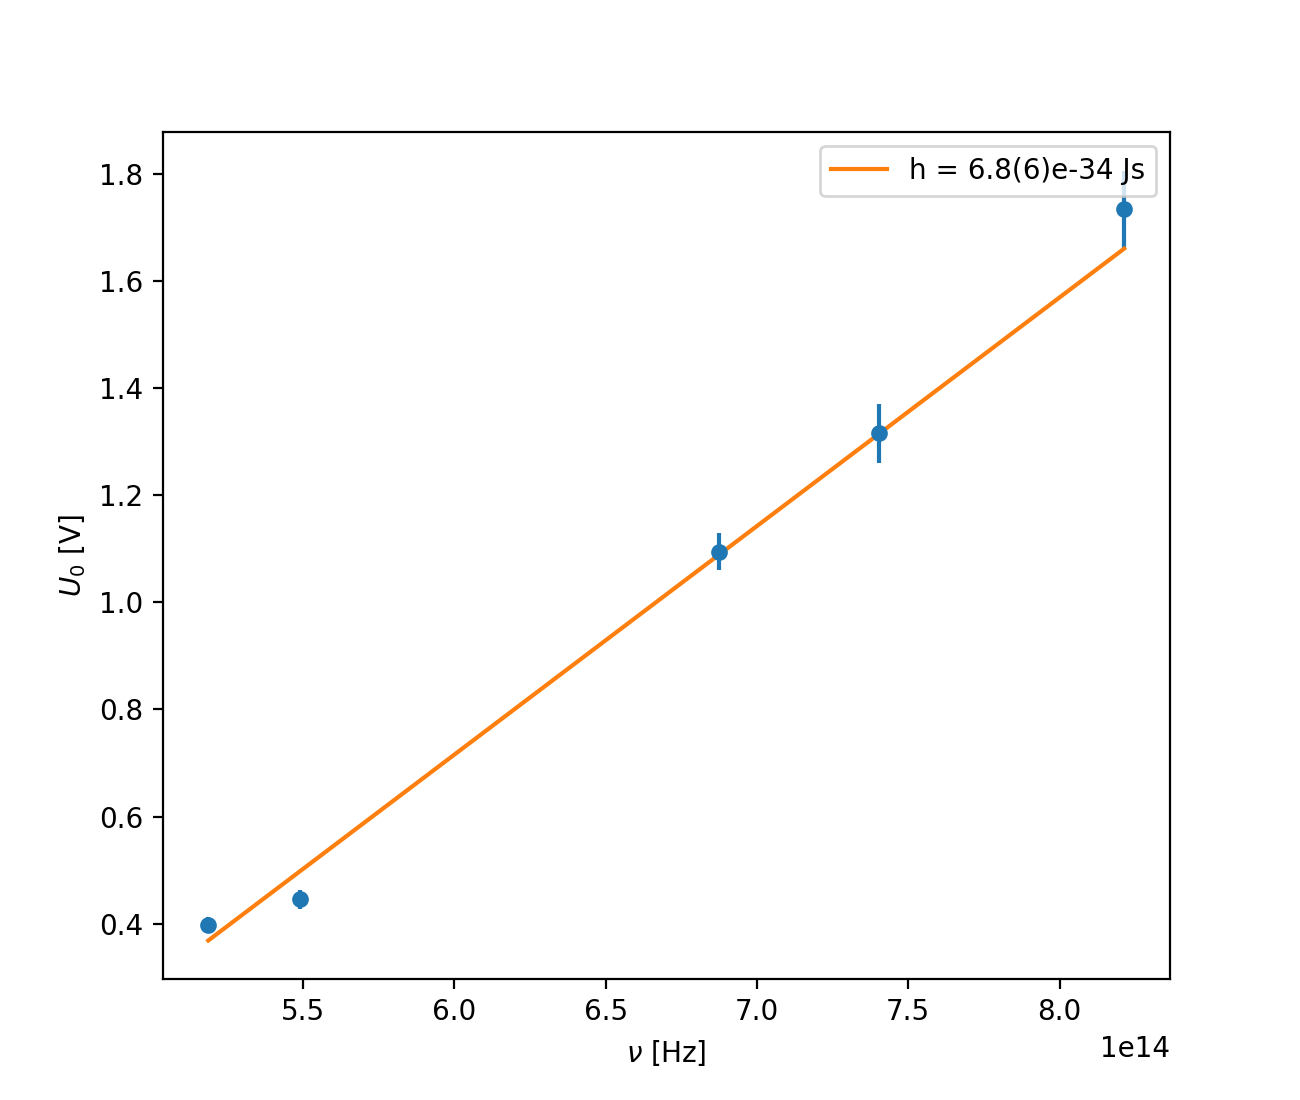
\includegraphics[width=0.75\linewidth]{../figs/photozelle_wirkungsquantum.png}
	\caption{Bestimmung des Planckschen Wirkungsquantums}
	\label{fig:bestimmung_planck}
\end{figure}

Die Grenzspannungen lassen sich jetzt gegen die Lichtfrequenz auftragen, die mit
der Relation $\nu = \mathrm c / \lambda$ berechnet wird. Aus \cref{eq:gegenfeldmethode} lässt sich
ablesen, dass aus der Steigung $m$ das Plancksche Wirkungsquantum bestimmt werden kann mit
\begin{equation}
	\mathrm h = \mathrm e \cdot m,\qquad \Delta\mathrm h = \mathrm e \cdot \Delta m \nonumber
\end{equation}
und die Austritssarbeit der Anode aus dem Achsenabschnitt $b$ mit
\begin{equation}
	W_A = -\mathrm e \cdot b, \qquad -\mathrm e \cdot \Delta b . \nonumber
\end{equation}
Die Anpassungsgerade hat eine Güte $\chi^2/\mathrm{dof} = \num{20.05}$ und ist damit deutlich größer als
\num{1}. Dies ist zu kleinen Fehlern geschuldet, da visuell bewertet die Messpunke nicht auf einer
einheitlichen Linie liegen und insbesondere die Spannungen der kleinsten zwei Frequenzen eine im Vergleich
hohe Abweichung zur Anpassungsgeraden aufweisen, was zu erwarten war, da die Intensität
dieser Messung gering war mit starken Fluktuationen. Aus diesem Grund waren diese Messungen
am anfälligsten für Fehler, was sich hier wiederspiegelt.\\
Die bestimmten Parameter sind
\[m = \SI{4.00(17)e-15}{\volt\second},\qquad b = -\SI{1.75\pm .11}{\electronvolt}\]
und die sich daraus ergebenen Konstanten
\[\mathrm h = \SI{6.4(3)e-34}{\joule\second}, \qquad \mathrm W_{\mathrm A} = \SI{1.75\pm .11}{\electronvolt} .\]
Der Literaturwert des Planckschen Wirkungsquantums $\mathrm h = \SI{6.626}{\joule\second}$
liegt im $1\sigma$-Bereich der Messung, welche einen unter 5\%-igen Fehler aufweist.
Dieses Ergebnis ist damit im Rahmen dieses Versuchs zufriedenstellend. Im Vergleich 
zu den Messfehlern der Kennlinie ist jedoch die Unsicherheit des Wirkungsquantums 
groß ausgefallen. Wie schon erwähnt ist der Grund hierfür die Abweichungen 
der Grenzspannungen für kleinere Frequenzen. Dies ist mit hoher Wahrscheinlichkeit der 
Versuchsdurchführung geschuldet, da für diese Frequenzen eine vergleichbar geringe 
Intensität gemessen wurde. Für \SI{578}{\nano\meter} lag die maximale Messung bei \SI{85\pm 5}{\pico\ampere}
und die Grenzspannung wurde schon bei etwa \SI{370\pm 10}{\milli\volt} erreicht, obwohl
am Spannungsteiler ein Maximum von \SI{2.77}{\volt} eingestellt war.
Um die Messung empflindlicher einzustellen, hätte es sich angeboten, mit einer 
Reihenschaltung von Widerständen die maximale Spannung weiter zu minimieren.\\

Zur Anodenaustrittsarbeit einer Platin-Rhodium-Elektrode
konnte kein Literaturwert zum Vergleich herbeigezogen werden, im Vergleich
zu anderen Werten oft genutzter Elemente\cite{wiki:austrittsarbeit} ist dieser Wert in der
gleichen Größenordnung. Dennoch verwunderlich ist, dass die genutzte Kalium
Kathode eine Austrittsarbeit von \SI{2.25}{\electronvolt}\cite{wiki:austrittsarbeit}
besitzt und da die Kathode von Prinzip eine geringere Bindungsenergie
haben sollte, stellt die Messung einen Widerspruch dazu auf. Eine mögliche
Fehlerquelle sei hierbei die Raumtemperatur bei der Durchführung.
Die zu messende Energie ist die Austritsarbeit bei der Annahme, dass sich 
die Elektronen in der Elektrode im Grundzustand befinden. Dies ist 
bei Temperaturen $T>0$ nicht der Fall, wodurch bei hohen Temperaturen
die Bindungsenergie verringert und das Messergebnis verfälscht wird. 
Für eine genauere Messung der Austritssarbeit ist eine Abkühlung 
der Photozelle unumgänglich, was im Rahmen dieses Versuchs nicht möglich war.\\\par

\doublefigure{365_3}{365_4}{365}{bei hoher Intensität}
\begin{figure}[htbp]
   \centering
\caption{Kennlinie \SI{365}{nm} hohe Intensität}
\begin{tabular}{cc||cc}
\hline\multicolumn{2}{c||}{erste Messung} & \multicolumn{2}{c}{zweite Messung}\\

\hline
$U / \unit{\milli\volt}$ & $I / \unit{\pico\ampere}$ & $U / \unit{\milli\volt}$ & $I / \unit{\pico\ampere}$ \\ 
\hline
$\num{0}$ & $\num{1150\pm 10}$ & $\num{0}$ & $\num{1100\pm 50}$ \\
$\num{57}$ & $\num{1050\pm 10}$ & $\num{76}$ & $\num{1000\pm 10}$ \\
$\num{136}$ & $\num{940\pm 20}$ & $\num{249}$ & $\num{770\pm 20}$ \\
$\num{199}$ & $\num{860\pm 10}$ & $\num{497}$ & $\num{480\pm 10}$ \\
$\num{280}$ & $\num{750\pm 10}$ & $\num{724}$ & $\num{305\pm 2}$ \\
$\num{357}$ & $\num{630\pm 20}$ & $\num{911}$ & $\num{174\pm 4}$ \\
$\num{440}$ & $\num{560\pm 10}$ & $\num{1118}$ & $\num{81\pm 2}$ \\
$\num{550}$ & $\num{440\pm 10}$ & $\num{1293}$ & $\num{34\pm 2}$ \\
$\num{697}$ & $\num{320\pm 5}$ & $\num{1406}$ & $\num{15\pm 1}$ \\
$\num{878}$ & $\num{180\pm 5}$ & $\num{1487}$ & $\num{-1.0\pm 0.5}$ \\
$\num{1066}$ & $\num{92\pm 1}$ & $\num{1592}$ & $\num{-17.4\pm 0.2}$ \\
$\num{1159}$ & $\num{62\pm 4}$ & $\num{1692}$ & $\num{-21.9\pm 0.1}$ \\
$\num{1331}$ & $\num{27\pm 3}$ & $\num{1888}$ & $\num{-22.2\pm 0.1}$ \\
$\num{1444}$ & $\num{7.5\pm 0.5}$ & $\num{2783}$ & $\num{-22.6\pm 0.2}$ \\
$\num{1497}$ & $\num{-4.5\pm 0.5}$ &    &    \\
$\num{1568}$ & $\num{-15.5\pm 0.1}$ &    &    \\
$\num{1640}$ & $\num{-20.8\pm 0.2}$ &    &    \\
$\num{1888}$ & $\num{-22.9\pm 0.1}$ &    &    \\
$\num{2783}$ & $\num{-23.2\pm 0.1}$ &    &    \\
\hline\end{tabular}
\label{kennlinie_365nm_hohe_intensität}
\end{figure}

Als Letztes wird der Intensitätseinfluss auf die Kennlinie bei \SI{365}{\nano\meter}
untersucht. Die Linien bei erhöhter Lichtintensität sind in \cref{fig:kennlinie_365bei hoher Intensität}
abgebildet. Da bei höherer Lichteinstrahlung mehr Photonen
auf die Kathode treffen muss der Photostrom ansteigen, da
aber die Energie der einzelnen Teilchen gleich bleibt, darf sich
die Grenzspannung nicht verändern.\\
Dieses Verhalten ist auch hier zu beobachten. Bei Vergleich von \cref{kennlinie_365nm} mit
\cref{fig:kennlinie_365bei hoher Intensität} wird ersichtlich, dass
bei geringerer Intensität ein maximaler Strom von etwa \SI{730}{\pico\ampere} gemessen
wurde und bei erhöhter Lichteinstrahlung \SI{1100}{\pico\ampere} (siehe
\cref{kennlinie_365nm_hohe_intensität}).\\

Die Ausgleichsgeraden haben eine Güte von $\chi^2_1/\mathrm{dof} = \num{0.14}$ und
$\chi^2_2/\mathrm{dof} = \num{0.36}$ und sind damit vergleichbar gut wie für die restlichen
Kennlinien (siehe \cref{fig:messwerte_grenzspannungen}). Beide besitzen eine gemittelte
Grenzspannung von \SI{1540\pm43}{\milli\volt}, was verglichen mit \SI{1556\pm 15}{\milli\volt}
aus \cref{fig:messwerte_grenzspannungen} im $1\sigma$-Fehlerbereich liegt. \\
Damit kann die Schlussfolgerung getroffen werden, dass die Grenzspannung
bei fester Wellenlänge des einstrahlenden Lichts nicht von der Intensität abhängt.
